\documentclass[a4paper,12pt]{article} 
\usepackage[left=2.5cm,right=1cm,top=2.5cm,bottom=2cm]{geometry}
%%% Работа с русским языком
\usepackage{cmap}					% поиск в PDF
%\usepackage{mathtext} 				% русские буквы в фомулах
\usepackage[T2A]{fontenc}			% кодировка
\usepackage[utf8]{inputenc}			% кодировка исходного текста
\usepackage[english,russian]{babel}	% локализация и переносы
\usepackage{amsmath} 
\usepackage{float}
\usepackage{graphicx}
\graphicspath{ {./images/} }
\usepackage{hyperref}
\hypersetup{				% Гиперссылки
    unicode=true,           % русские буквы в раздела PDF
    colorlinks=true,        % false: ссылки в рамках; true: цветные ссылки
    linkcolor=black,        % внутренние ссылки
    citecolor=black,        % на библиографию
    filecolor=magenta,      % на файлы
    urlcolor=blue           % на URL
}

% \usepackage{tocbasic}
% \renewcommand*{\listoffigures}{\listoftoc[\listfigurename]{lof}}
% \renewcommand*{\listoftables}{\listoftoc[\listtablename]{lot}}
% % \setuptoc{lof}{leveldown,totoc}
% % \setuptoc{lot}{leveldown,totoc}

%%% Дополнительная работа с математикой
\usepackage{amsmath,amsfonts,amssymb,amsthm,mathtools} % AMS
\usepackage{icomma} % "Умная" запятая: $0,2$ --- число, $0, 2$ --- перечисление

%% Номера формул
%\mathtoolsset{showonlyrefs=true} % Показывать номера только у тех формул, на которые есть \eqref{} в тексте.

\usepackage{cite} % Работа с библиографией
%\usepackage[superscript]{cite} % Ссылки в верхних индексах
%\usepackage[nocompress]{cite} % 
\usepackage{csquotes} % Еще инструменты для ссылок
\usepackage{listings} % For code highlithing
\usepackage{xcolor}

\definecolor{codegreen}{rgb}{0,0.6,0}
\definecolor{codegray}{rgb}{0.5,0.5,0.5}
\definecolor{codepurple}{rgb}{0.58,0,0.82}
\definecolor{backcolour}{rgb}{0.95,0.95,0.92}

\lstdefinestyle{mystyle}{
    backgroundcolor=\color{backcolour},   
    commentstyle=\color{codegreen},
    keywordstyle=\color{magenta},
    numberstyle=\tiny\color{codegray},
    stringstyle=\color{codepurple},
    basicstyle=\ttfamily\footnotesize,
    breakatwhitespace=false,         
    breaklines=true,                 
    captionpos=b,                    
    keepspaces=true,                 
    numbers=left,                    
    numbersep=5pt,                  
    showspaces=false,                
    showstringspaces=false,
    showtabs=false,                  
    tabsize=2
}
\lstset{style=mystyle}
\lstset{extendedchars=\true}
\begin{document} % конец преамбулы, начало документа
%\pagestyle{empty} 
\thispagestyle{empty}

\begin{center}
    {\huge
    Частное общеобразовательное учреждение
    
    <<Школа разговорных языков>>
    }
    \vfill
    \vfill
    \vfill
    \vfill
    {\huge \textsc{ПРОЕКТ}}
    \vfill
    {\huge на тему}
    \vfill
{\huge \textsc{\textbf{«Вычисление значения $\pi$.}}}

\vspace{0.5cm}

{\huge \textsc{\textbf{Численное интегрирование.}}}

\vspace{0.5cm}

{\huge \textsc{\textbf{Метод прямоугольников»}}}

\vfill
{\huge (по Информатике и ИКТ)}

\vfill 
    
    \begin{flushright}
    {\Large ученика 11 класса 
    
    \vspace{0.5cm}

    Доричева Тимофея Константиновича}
    \end{flushright}
    \vfill
    {\Large Санкт-Петербург
    
    \vspace{0.5cm}

    2024}
\end{center}
\pagebreak

\tableofcontents

\section{Введение}

Цель данного проекта~--- наглядно пояснить один из численных методов вычисления значения $\pi$~--- метод прямоугольников.

Работа выполнена с использованием языка программирования \href{https://www.python.org/}{Python}, библиотек \href{https://numpy.org/}{NumPy}, \href{https://matplotlib.org/}{Matplotlib}, \href{https://seaborn.pydata.org/}{Seaborn}. 

Работа оформлена в~издательской системе \href{https://ru.wikipedia.org/wiki/LaTeX}{\LaTeX}.


\section{Краткая историческая справка}

Число $\pi$ (произносится «пи») — математическая постоянная, равная отношению длины окружности к её диаметру.

Число $\pi$ иррационально, то есть его значение не может быть точно выражено в виде дроби 
$ \frac {m}{n}$, где 
$m$~--- целое число, а $n$~--- натуральное. Следовательно, его десятичное представление никогда не заканчивается и не является периодическим. 

Иррациональность числа $\pi$ была впервые доказана Иоганном Ламбертом в 1761 году путём разложения тангенса в непрерывную дробь.

Первые 50 знаков мантиссы числа $\pi$ \cite[Википедия]{wiki}:

\begin{align}\label{eq:pi_50}
\pi \approx 3.14159265358979323846264338327950288419716939937510\ldots
\end{align}

\pagebreak

\section{Теоретическое обоснование используемого метода}

Общеизвестно, что площадь круга S вычисляется по формуле:

\begin{align}\label{eq:circle_square}
    S = \pi \times R^2
\end{align}

где R~--- радиус круга

Из \ref{eq:circle_square} имеем:

\begin{align}\label{eq:pi1}
\pi = \frac{S}{R^2} 
\end{align}

А для окружности единичного радиуса ($R = 1$),

\begin{align}\label{eq:pi}
    \pi = S
\end{align}

Также общеизвестно, что уравнение окружности в декартовой системе координат имеет вид:

\begin{align}\label{eq:circle}
    x^2 + y^2 = R^2
\end{align}

А для единичной окружности в первой четверти декартовой системы координат:

\begin{align}\label{eq:y}
    y = \sqrt{1-x^2}, x \in [0,1]
\end{align}

Таким образом, площадь \textit{четверти} круга будет численно равна площади фигуры, ограниченной осями координат и графиком функции \ref{eq:y}.

Данную площадь можно вычислить с помощью определённого интеграла:
\begin{align}\label{eq:s_4}
S/4 = \int_{0}^{1} \sqrt{1-x^2} \,dx 
\end{align}

Тогда, из \ref{eq:pi} и \ref{eq:s_4} имеем окончательную рабочую расчётную формулу:

\begin{align}\label{eq:pi_final}
    \pi = 4 \times \int_{0}^{1} \sqrt{1-x^2} \,dx 
\end{align}

\section{Суть метода прямоугольников}

Для нахождения значения интеграла \ref{eq:pi_final} воспользуемся методом прямоугольников. Суть метода состоит в разбиении интервала интегрирования на равные промежутки и аппроксимации приращения функции на интервале константой. 
Далее находятся и суммируются площади полученных прямоугольников, и при количестве интервалов разбиения $ n \rightarrow \infty $, полученное значение стремится к значению интеграла.

В зависимости от того, какое значение функции принимают за основу, различают методы левых, правых и серединных прямоугольников.

\begin{figure}[h]
    \begin{center}
    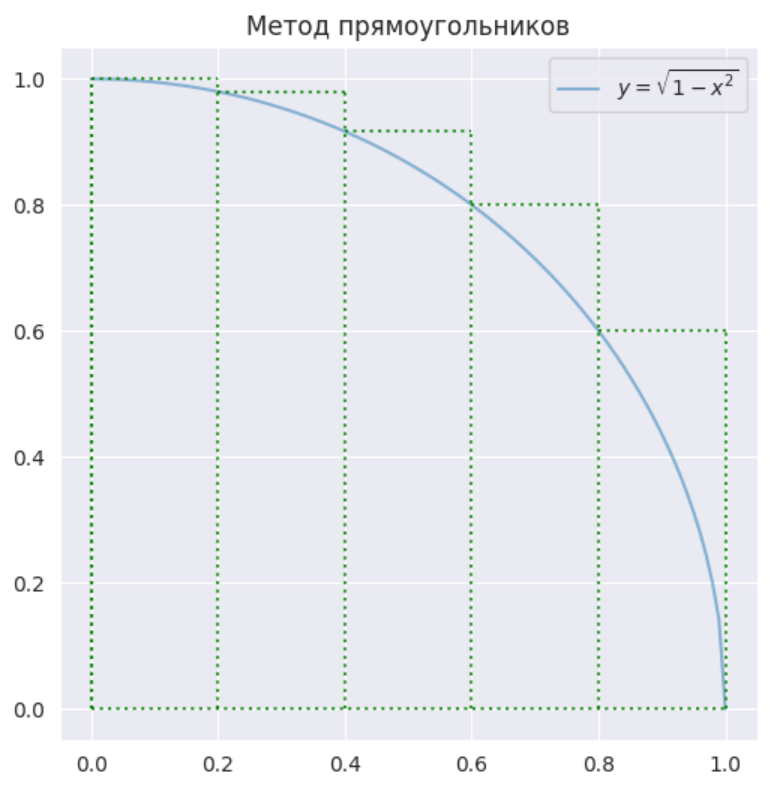
\includegraphics[width=12cm]{rect.png}    
    \caption{Метод левых прямоугольников}
    \label{left_rect}
    \end{center}
\end{figure}

Так, для любого элементарного интервала $[a,b]$ и метода \textit{левых} прямоугольников имеем:

\begin{align}\label{eq:rect_approx}
    \int_{a}^{b} f(x)\,dx \approx f(a)\times (b-a)
\end{align}

Тогда из \ref{eq:pi_final}, заменив интеграл суммой, имеем:

\begin{align}\label{eq:pi_sum}
    \pi = 4 \times \int_{0}^{1} \sqrt{1-x^2} \,dx \approx 4 \times \sum_{n = 0}^{n-1} f(x_i)\times(x_{i+1}-x_i)
\end{align}

Подробнее метод описан в \cite{rect}.

\section{Расчёты}

Для вычисления (\ref{eq:pi_sum}) напишем на языке программирования Python функцию, которая будет принимать на вход аргумент n~--- количество интервалов интегрирования (num\_intervals) и возвращать значение $\pi$ и разницу с известным, базовым значением~--- ошибку. За базовое возьмём значение, используемое в библиотеке NumPy:

$$\pi \approx 3.141592653589793$$

Точность~--- 15 знаков мантиссы, сравни с (\ref{eq:pi_50}).


\begin{lstlisting}[language=Python, caption=Функция вычисления $\pi$ и ошибки]
import numpy as np

def pi_rectangles(num_intervals: int) -> tuple[np.float64, np.float64]:

    if num_intervals == 0:
        return np.NaN, np.NaN
    
    dx = np.double(1.0) / num_intervals
    x = np.linspace(0, 1, num_intervals, endpoint=False)
    y = np.sqrt(1 - x**2)
    ds = y * dx
    pi = np.sum(ds) * 4
    return pi, pi - np.pi    
\end{lstlisting}    

Необходимо отметить, что библиотека NumPy поддерживает т.\ н. векторизацию~--- один из способов реализации параллельных вычислений. Поэтому позволяет писать эффективный и компактный код и в некоторых случаях, как выше, избегать циклов, работая с векторами.

Так, к примеру, строка 7 листинга 1~--- получение вектора значений аргумента $x$, а строки 8, 9~--- вычисление всех значений функции $y$ во всех точках $x$, и всех значений площадей прямоугольников $ds$.


\section{Анализ полученных результатов}

В таблице \ref{table:results} приведены вычисленные значения константы $\pi$ в зависимости от количества интервалов интегрирования $n$~--- количества прямоугольников, а также значения ошибки. Жирным шрифтом выделены верные цифры.

\begin{table}[h!]
    \caption{Результаты вычислений\label{table:results}}
    \begin{center}
    \begin{tabular}{||r l l||} 
     \hline
     n & Значение $\pi$ & Ошибка \\ [0.5ex] 
     \hline\hline
     1       & 4.0                        & 0.858407346410207 \\ 
     \hline
     10      & \textbf{3}.304518326248318 & 0.162925672658520 \\
     \hline
     100     & \textbf{3.1}60417031779045 & 0.018824378189252 \\
     \hline
     1000    & \textbf{3.14}3555466911028 & 0.001962813321235 \\ 
     \hline
     10000   & \textbf{3.141}791477611323 & 0.000198824021529 \\ 
     \hline
     100000  & \textbf{3.141}612616401987 & 0.000019962812194 \\ 
     \hline
     1000000 & \textbf{3.14159}4652413811 & 0.000001998824017 \\ 
     \hline               
    \end{tabular}
    \end{center}
\end{table}

\begin{figure}[h]\
    \begin{center}
    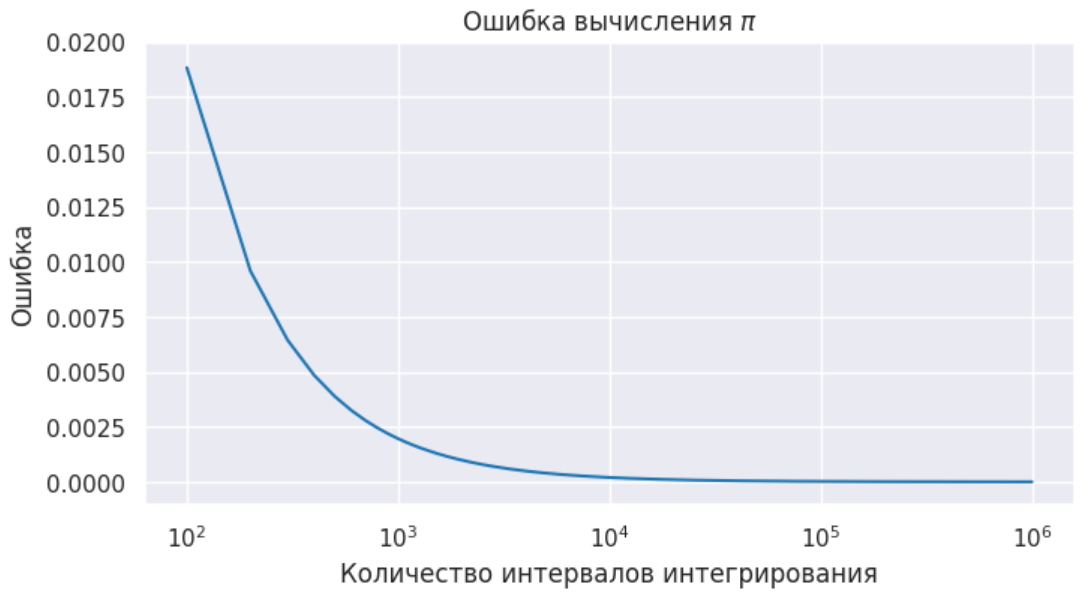
\includegraphics[width=\textwidth]{error.png}    
    \caption{Ошибка вычислений как функция количества интервалов интегрирования}
    \label{fig:error}
    \end{center}
\end{figure}

На рисунке~\ref{fig:error} ось абсцисс для наглядности выбрана в логарифмическом масштабе.

\section{Заключение}

В данной работе продемонстрирован один из численных методов вычисления значение константы $\pi$~--- метод прямоугольников.

\pagebreak

\section{Приложение. Код построения графика}

\begin{lstlisting}[language=Python, caption=Код построения рис.\ref{left_rect}]
    import numpy as np
    import matplotlib.pyplot as plt
    import seaborn as sns

    # Значения функции
    x = np.linspace(0, 1, 100, endpoint=True)
    y = np.sqrt(1 - x**2)

    # Значения функции для прямоугольников
    xr = np.linspace(0, 1, 5, endpoint=False)
    yr = np.sqrt(1 - xr**2)

    # Построение графика
    fig, ax = plt.subplots(figsize=(6, 6))
    sb_ax = sns.lineplot(y=y, x=x,alpha=0.5, label="$y = \sqrt{1 - x^2}$")
    sb_ax.set(title = 'Метод прямоугольников')
    ax.set_xlim(-0.05,1.05)
    ax.set_ylim(-0.05,1.05)

    # Построение прямоугольников
    sb_ax.hlines(
        y=yr,
        xmin=xr[:],
        xmax=[*xr[1:], 1.0],
        colors='green',
        linestyles='dotted',
        alpha=0.8,
    )
    sb_ax.vlines(
        x=[*xr, 1.0],
        ymin=0,
        ymax=[1.0, *yr[:]],
        colors='green',
        linestyles='dotted',
        alpha=0.8,
    )
    ax.vlines(
        x=0.0,
        ymin=0,
        ymax=1.0,
        colors='green',
        linestyles='dotted',
        alpha=0.8,
    )
    ax.hlines(
        y=0.0,
        xmin=0,
        xmax=1.0,
        colors='green',
        linestyles='dotted',
        alpha=0.8,
    )    
\end{lstlisting}

\addcontentsline{toc}{section}{Список иллюстраций}

\listoffigures

\addcontentsline{toc}{section}{Список таблиц}
\listoftables

\begin{thebibliography}{9}
    \addcontentsline{toc}{section}{\refname}

    \bibitem{wiki}\href{https://ru.wikipedia.org/wiki/%D0%9F%D0%B8_(%D1%87%D0%B8%D1%81%D0%BB%D0%BE)}{Википедия. Число Пи}  

    \bibitem{rect}\href{https://ru.wikipedia.org/wiki/%D0%9C%D0%B5%D1%82%D0%BE%D0%B4_%D0%BF%D1%80%D1%8F%D0%BC%D0%BE%D1%83%D0%B3%D0%BE%D0%BB%D1%8C%D0%BD%D0%B8%D0%BA%D0%BE%D0%B2}{Википедия. Метод прямоугольников}

    \bibitem{numpy}Библиотека Numerical Python (NumPy). \href{https://numpy.org/}{numpy.org}

    \bibitem{seaborn}Графическая библиотека Seaborn. \href{https://seaborn.pydata.org/generated/seaborn.lineplot.html}{seaborn.pydata.org}
\end{thebibliography}

\end{document}
